%   Filename    : chapter_3.tex
% \section*{Chapter 3}\label{sec:researchmethod}
\chapter{Research Methodology}

This chapter outlines and explains the specific steps and activities to be carried out in completing the project.

\section{Research Activities}

As illustrated in \figref{fig:process_diagram}, the researchers will carry out a sequence of computational procedures designed to detect PCR-induced chimeric reads in mitochondrial genomes. The process begins with the collection of mitochondrial reference sequences from the NCBI database, which will serve as the foundation for generating simulated chimeric reads. These datasets will then undergo bioinformatics pipeline development, which includes alignment, k-mer extraction, and homology-based filtering to prepare the data for model construction. The machine-learning model will subsequently be trained and tested using the processed datasets to assess its accuracy and reliability. Depending on the evaluation results, the model will either be refined and retrained to improve performance or, if the metrics meet the desired threshold, deployed for further validation and application.

\begin{figure}[H]
  \centering
  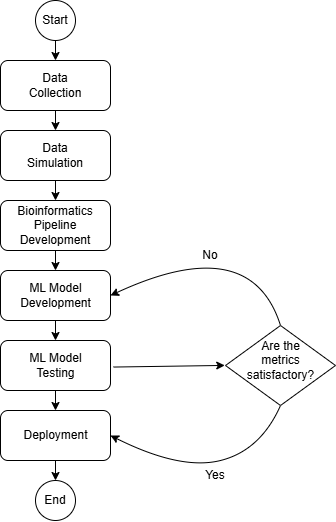
\includegraphics[width=0.4\linewidth]{figures/research_activities.png}
  \caption{Process Diagram of Special Project}\label{fig:process_diagram}
\end{figure}

\subsection{Data Collection}

The researchers will collect mitochondrial genome reference sequences of \textit{Sardinella lemuru} from the National Center for Biotechnology Information (NCBI) database. The downloaded files will be in FASTA format to ensure compatibility with bioinformatics tools and subsequent analysis. The gathered sequences will serve as the basis for generating simulated chimeric reads to be used in model development.

The expected outcome of this process is a comprehensive dataset of \textit{Sardinella lemuru} mitochondrial reference sequences that will serve as the foundation for the succeeding stages of the study. This step is scheduled to start in the first week of November~2025 and is expected to be completed by the last week of November~2025, with a total duration of approximately one (1) month.

\subsection{Data Simulation}

The researchers will simulate sequencing data using the reference sequences collected from NCBI. Using \texttt{wgsim}, a total of 5{,}000 paired-end reads (R1 and R2) will be generated from the reference genome and designated as clean reads. These reads will be saved in FASTQ (\texttt{.fastq}) format. From the same reference, a Bash script will be created to deliberately cut and reconnect portions of the sequence, introducing artificial junctions that mimic chimeric regions. The manipulated reference file, saved in FASTA (\texttt{.fasta}) format, will then be processed in \texttt{wgsim} to simulate an additional 5{,}000 paired-end chimeric reads, also stored in FASTQ (\texttt{.fastq}) format. The resulting read files will be aligned to the original reference genome using SAMtools, generating SAM (\texttt{.sam}) or BAM (\texttt{.bam}) alignment files. During this alignment process, clean reads will be labeled as ``0,'' while chimeric reads will be labeled as ``1'' in a corresponding CSV (\texttt{.tsv}) file.

The expected outcome of this process is a complete set of clean and chimeric paired-end reads prepared for subsequent analysis and model development. This step is scheduled to start in the first week of November~2025 and is expected to be completed by the last week of November~2025, with a total duration of approximately one (1) month.

\subsection{Bioinformatics Tools Pipeline}

The researchers will obtain the necessary analytical features through the development and implementation of a bioinformatics pipeline. This pipeline will serve as a reproducible and modular workflow that accepts FASTQ and BAM inputs, processes these through a series of analytical stages, and outputs tabular feature matrices (TSV) for downstream machine learning. All scripts will be version-controlled through GitHub, and computational environments will be standardized using Conda to ensure cross-platform reproducibility. To promote transparency and replicability, the exact software versions, parameters, and command-line arguments used in each stage will be documented. To further ensure correctness and adherence to best practices, the researchers will consult with bioinformatics experts in Philippine Genome Center Visayas for validation of pipeline design, feature extraction logic, and overall data integrity. This stage of the study is scheduled to begin in the last week of November~2025 and conclude by the last week of January~2026, with an estimated total duration of approximately two (2) months.

The bioinformatics pipeline focuses on three principal features from the simulated and aligned sequencing data: (1) supplementary alignment count (SA count), (2) k-mer composition difference between read segments, and (3) micro-homology length at potential junctions. Each of these features captures a distinct biological or computational signature associated with PCR-induced chimeras.

\subsubsection{Alignment and Supplementary Alignment Count}
This will be derived through sequence alignment using Minimap2, with subsequent processing performed using SAMtools and \texttt{pysam} in Python. Sequencing reads will be aligned to the \textit{Sardinella lemuru} mitochondrial reference genome using Minimap2 with the \texttt{-ax sr} preset (optimized for short reads). The output will be converted and sorted using SAMtools, producing an indexed BAM file which will be parsed using \texttt{pysam} to count the number of supplementary alignments (SA tags) per read. Each read’s mapping quality, number of split segments, and alignment characteristics will be recorded in a corresponding TSV file. The presence of multiple alignment loci within a single read, as reflected by a nonzero SA count, serves as direct computational evidence of chimerism. Reads that contain supplementary alignments or soft-clipped regions are strong candidates for chimeric artifacts arising from PCR template switching or improper assembly during sequencing.

\subsubsection{K-mer Composition Difference}
Chimeric reads often comprise fragments from distinct genomic regions, resulting in a compositional discontinuity between segments. Comparing k-mer frequency profiles between the left and right halves of a read allows detection of such abrupt compositional shifts, independent of alignment information. This will be obtained using Jellyfish, a fast k-mer counting software. For each read, the sequence will be divided into two segments, either at the midpoint or at empirically determined breakpoints inferred from supplementary alignment data, to generate left and right sequence segments. Jellyfish will then compute k-mer frequency profiles (with $k = 5$ or $6$) for each segment. The resulting k-mer frequency vectors will be normalized and compared using distance metrics such as cosine similarity or Jensen–Shannon divergence to quantify compositional disparity between the two halves of the same read. The resulting difference scores will be stored in a structured TSV file.

\subsubsection{Micro-homology Length}
The micro-homology length will be computed using a custom Python script that detects the longest exact suffix–prefix overlap within $\pm 30$ base pairs surrounding a candidate breakpoint. This analysis identifies the number of consecutive bases shared between the end of one segment and the beginning of another. The presence and length of such micro-homology are classic molecular signatures of PCR-induced template switching, where short identical regions (typically 3–15 base pairs) promote premature termination and recombination of DNA synthesis on a different template strand. By quantifying micro-homology, the researchers can assess whether the suspected breakpoint exhibits characteristics consistent with PCR artifacts rather than true biological variants. Each read will therefore be annotated with its corresponding micro-homology length, overlap sequence, and GC content.

After extracting the three primary features, all resulting TSV files will be joined using the read identifier as a common key to generate a unified feature matrix. Additional read-level metadata such as read length, mean base quality, and number of clipped bases will also be included to provide contextual information. This consolidated dataset will serve as the input for subsequent machine-learning model development and evaluation.

\subsection{Machine-Learning Model Development}

The classification component of MitoChime will employ two ensemble algorithms—Random Forest (RF) and Extreme Gradient Boosting (XGBoost)—to evaluate complementary learning paradigms. Random Forest applies bootstrap aggregation (bagging) to reduce model variance and improve stability, whereas XGBoost implements gradient boosting to minimize bias and capture complex non-linear relationships among genomic features. Using both models enables a balanced assessment of predictive performance and interpretability.

The dataset will be divided into training (80\%) and testing (20\%) subsets. The training data will be used for model fitting and hyperparameter optimization through five-fold cross-validation, in which the data are partitioned into five folds; four folds are used for training and one for validation in each iteration. Performance metrics will be averaged across folds, and the optimal parameters will be selected based on mean cross-validation accuracy. The final models will then be evaluated on the held-out test set to obtain unbiased performance estimates.

Model development and evaluation will be implemented in Python (version~3.11) using the \texttt{scikit-learn} and \texttt{xgboost} libraries. Standard metrics including accuracy, precision, recall, F1-score, and area under the ROC curve (AUC) will be computed to quantify predictive performance. Feature-importance analyses will be performed to identify the most discriminative variables contributing to chimera detection.

\subsection{Validation and Testing}

Validation will involve both internal and external evaluations. Internal validation will be achieved through five-fold cross-validation on the training data to verify model generalization and reduce variance due to random sampling. External validation will be achieved through testing on the 20\% hold-out dataset derived from the simulated reads, which will serve as an unbiased benchmark to evaluate how well the trained models generalize to unseen data. All feature extraction and preprocessing steps will be performed using the same bioinformatics pipeline to ensure consistency and comparability across validation stages.

Comparative evaluation between the Random Forest and XGBoost classifiers will establish which model achieves superior predictive accuracy and computational efficiency under identical data conditions.

\subsection{Documentation}

Comprehensive documentation will be maintained throughout the study to ensure transparency, reproducibility, and scientific integrity. All stages of the research—including data acquisition, preprocessing, feature extraction, model training, and validation—will be systematically recorded. For each analytical step, the corresponding parameters, software versions, and command-line scripts will be documented to enable exact replication of results.

Version control and collaborative management will be implemented through GitHub, which will serve as the central repository for all project files, including Python scripts, configuration settings, and Jupyter notebooks. The repository structure will follow standard research data management practices, with clear directories for datasets, processed outputs, and analysis scripts. Changes will be tracked through commit histories to ensure traceability and accountability.

Computational environments will be standardized using Conda, with environment files specifying dependencies and package versions to maintain consistency across systems. Experimental workflows and exploratory analyses will be conducted in Jupyter Notebooks, which facilitate real-time visualization, annotation, and incremental testing of results.

For the preparation of the final manuscript and supplementary materials, Overleaf (LaTeX) will be utilized to produce publication-quality formatting, consistent referencing, and reproducible document compilation. The documentation process will also include a project timeline outlining major milestones such as data collection, simulation, feature extraction, model evaluation, and reporting to ensure systematic progress and adherence to the research schedule.

\section{Calendar of Activities}

Table~\ref{tab:project_timeline} presents the project timeline in the form of a Gantt chart, where each bullet point corresponds to approximately one week of planned activity.

\begin{table}[H]
  \centering
  \caption{Timetable of Activities}\label{tab:project_timeline}
  \resizebox{\textwidth}{!}{%
    \begin{tabular}{|c|c|c|c|c|c|c|c|}
      \hline
      \textbf{Activities (2025)} & \textbf{Nov} & \textbf{Dec} & \textbf{Jan} & \textbf{Feb} & \textbf{Mar} & \textbf{Apr} & \textbf{May} \\
      \hline
      Data Collection and Simulation & $\bullet\bullet\bullet\bullet$ &  &  &  &  &  &  \\
      \hline
      Bioinformatics Tools Pipeline & $\bullet\bullet$ & $\bullet\bullet\bullet\bullet$ & $\bullet\bullet\bullet\bullet$ &  &  &  &  \\
      \hline
      Machine Learning Development &  &  & $\bullet\bullet$ & $\bullet\bullet\bullet\bullet$ & $\bullet\bullet\bullet\bullet$ & $\bullet\bullet$ &  \\
      \hline
      Testing and Validation &  &  &  &  &  & $\bullet\bullet$ & $\bullet\bullet\bullet\bullet$ \\
      \hline
      Documentation & $\bullet\bullet\bullet\bullet$ & $\bullet\bullet\bullet\bullet$ & $\bullet\bullet\bullet\bullet$ & $\bullet\bullet\bullet\bullet$ & $\bullet\bullet\bullet\bullet$ & $\bullet\bullet\bullet\bullet$ & $\bullet\bullet\bullet\bullet$ \\
      \hline
    \end{tabular}%
  }
\end{table}